\documentclass[journal,10pt,onecolumn,compsoc]{IEEEtran} \usepackage[margin=1.0in]{geometry} \usepackage{pdfpages} 
\usepackage{caption,graphicx,float} 
\usepackage{listings}
\usepackage{verbatim}
\usepackage{url}
\graphicspath{/graphics} \setlength{\parskip}{\baselineskip} \setlength\parindent{24pt}
\usepackage[english]{babel}
%\usepackage{fullpage}

\title{TensorFlow\texttrademark WYSIWYG GUI Design Document}
\author{Group 33: Connor Sedwick, Behnam Saeedi, Collin Dorsett}
\date{\today}
\begin{document}
\maketitle
\begin{centering}
Fall 2016
\begin{abstract}
The purpose of this document is to discuss and outline the architecture and design choices made for the TensorFlow\texttrademark WYSIWYG Graphical User Interface system. 
The functionality and design choices made for  each component of the GUI is discussed in detail.
Also discussed is the reasoning behind the design choices made both from the viewpoint of the developers and from the viewpoint of the users.
\end{abstract}
\end{centering}
\newpage
\tableofcontents
\noindent\textbf{Apportioning of work:}\\
\noindent Every member of the design team contributed to each section in order to produce the complete picture rather than focusing on a specific portion.\\

\noindent\textbf{Connor Sedwick} contributed to: 
\begin{itemize}
	\item Base formatting for LaTeX document
	\item Sections: 
    \begin{itemize}
    \item Introduction \{Scope, Purpose, Reference Material\}, 
    \item System Overview, 
    \item System Architecture, 
    \item TensorFlow\texttrademark WYSIWYG GUI in Perspective
    \item Component Design
    \end{itemize}
    \item Architecture diagrams
\end{itemize}
\noindent\textbf{Behnam Saeedi} contributed to:
\begin{itemize}
	\item Figures
    \item Order of content
    \item glossary
    \item introduction
    \item TensorFlow\texttrademark WYSIWYG GUI in Perspective(Section \ref{TWYSIWYGGUI})
    \item component design: Probe, Blocks, Block Menu, Channels, Scene, Build, Run, Stop.
    \item References
\end{itemize}
\noindent\textbf{Collin Dorsett} contributed to:
\begin{itemize}
  \item Architectural Design
  \item Design Rationale
  \item Design Stakeholders and their Concerns
  \item Component Design: Extract, Channel, Probe
  \item Overview of User Interface
  \item Screen Objects and Actions
\end{itemize}

\newpage


\section{Introduction}
%---------------------------------------------
\subsection{Scope}
The software outlined in this document is meant to act as a development software used for machine learning.
Our goal is to develop a software that not only aids in the development of machine learning software, but will also act as a tool for teaching machine learning programming.
%---------------------------------------------
\subsection{Purpose}
The purpose of this Software Specification Document (SSD) is to provide an overview of how TensorFlow\texttrademark WYSIWYG GUI is designed.\cite{ieee}
To achieve this task, the document will outline and describe the architecture and functionality of the software.
\subsection{Intended Audience}
\noindent This document is intended for technical stakeholders who intend to produce a WYSIWYG interface for TensorFlow\texttrademark Machine learning API. 
This document guides the development team to be able to achieve the theoretical constructed solution in order to achieve software requirements and specifications. 
Furthermore, this document will be a reference for the developers, Capstone instructors and the stakeholder in case of any conflict of design and requirements.
\subsection{Conformance}
\noindent This document conforms with the stakeholders specifications and requirements provided to the design team by \today. Records of communications with the stakeholder is available in the developer and meeting attendee's journals.
%\subsection{Overview}
%---------------------------------------------
\subsection{Reference Material}

\noindent [1]"WYSIWYG - definition of WYSIWYG in English | Oxford Dictionaries", Oxford Dictionaries | English, 2016. [Online]. Available: https://en.oxforddictionaries.com/definition/WYSIWYG. [Accessed: 03- Nov- 2016].

\noindent [2]"What is graphical user interface (GUI)? definition and meaning", BusinessDictionary.com, 2016. [Online]. Available: http://www.businessdictionary.com/definition/graphical-user-interface-GUI.html. [Accessed: 03- Nov- 2016].

\noindent [3]Tensorflow.org, 2016. [Online]. Available: https://www.tensorflow.org/. [Accessed: 03- Nov- 2016]. 

%Put bibliography from Requirements Doc in here
%---------------------------------------------
\subsection{Definitions and Acronyms}
\begin{itemize}
	\item \textbf{WYSIWYG:}
		This is an abbreviation for "What You See Is What You Get".
		Microsoft PowerPoint and LibreOffice Impress are two good examples of such system. 
		In this system, the end result is very similar to user's preview of the output during the development.\\
	\item \textbf{Tensorflow\texttrademark:}
		TensorFlow\texttrademark is an open source software library for numerical computation using data flow graphs.
		TensorFlow\texttrademark was originally developed by researchers and engineers working on the Google Brain Team within Google's Machine Intelligence research organization for the purposes of 
		conducting machine learning and deep neural networks research, but the system is general enough to be applicable in a wide variety of other domains as well.\\
	\item \textbf{GUI:}
		GUI or Graphical User Interface, is an interface that allows users to interact with a given system through graphical icons as opposed to a text based, command-line representation.\\
	\item \textbf{Scene:}
		The work space where user can place different elements of their program.\\
	\item \textbf{Block:}
		A block is a GUI feature that represents a data structure or line of code. A block could be a variable, a constant, a method, a class, a probe, input or output.\\
	\item \textbf{Block-Menu:}
		A menu that contains all of the items and functionality icons that are ready to be dragged and dropped into the scene.\\
	\item \textbf{Run:}
		The task of starting the execution of a program.\\
	\item \textbf{Stop:}
		Brings the execution of the program to a halt. Resuming the process requires running the program again.
		This functionality will reset the state of the execution.\\
	\item \textbf{Extract:}
		A command that allows the user to pull the current version of their solution and save the file in a user-chosen space in memory.
		In order for a user to have a stand-alone version of their implemented program, they need to extract their project.\\
	\item \textbf{Variable/Constant:}
		Variables are equivalent to programming variables. They are represented by rhombuses in the graphical user interface.
		Constants are similar to  variables, however, these values can not be changed while running the program.
		Constants are also represented by rhombuses.\\
	\item \textbf{Method:}
		A function from the API that perform a specific task. They are represented by boxes.
		The circles on the edges of a method box are inputs and outputs of that method.\\
	\item \textbf{Class:} 
		An object that contains multiple variables and methods (public or private).
		Classes are represented as transparent boxes around methods and variables. This box could be abstracted away to be displayed as a solid color box.\\
	\item \textbf{Abstract:}
		A feature of a class that will turn the class from transparent to solid color in order to hide the content of the class.\\
	\item \textbf{Layer:} 
		An instance of a Scene. 
		These instances could be independently implemented so that they function individually.
		Layers can be run individually and they will generate data from input.\\
	\item \textbf{Channel:}
		 A connection between inputs and outputs that display the direction of data flow and route the data from one Block to another.\\
	\item \textbf{Probe:}
		A Block type that displays the content of a channel.
		Can modify the value which is being transmitted through the Channel it is placed on.
		If the value of a Probe is modified, the modification will happen after the point which the probe is inserted into the Channel.
		Every value that goes though the Channel before the probe is left unchanged with the exception of pointer Probes.\\
	\item \textbf{Input:}
		A Block type which allows the user to insert data into their program during the run process.\\
	\item \textbf{Output:}
		A Block type which allows the user to see the final result. Outputs indicate discontinuation of a Channel.\\
\end{itemize}
\newpage
%---------------------------------------------
\section{System Overview}
The TensorFlow\texttrademark WYSIWYG system is a software development tool. 
Currently, software developers working on machine learning projects do not have many resources available to them to aid them in visualizing neural networks.
The purpose of TensorFlow's WYSIWYG GUI is to facilitate the development and improve the readability of software during development.
Furthermore, it will abstract away some of the complexity and struggles of using syntax in order for user to create projects.

\noindent To improve readability, the WYSIWYG GUI displays a flowchart-styled mapping of a user's project.
The reasoning for this is to aid in the visualization of a software's architecture.
To achieve this the software has some specific functionality.
The WYSIWYG GUI supports a drag and drop interface which allows user's the ability to move items called Blocks around the project space.
User's are also provided the ability to draw connections between Blocks in order to set dependencies and control the flow of data.
When a user decides that they wish to test their algorithm, they can choose the option to Build their software based on the flowchart design they have created.
This option is a button that, once clicked, tells the software to interpret the architecture designed by the user and create a file containing code that provides the functionality of the user's design.
The user then can test their design by using the Run option which will load and run the interpreted file that was created.

\noindent During development some users may wish to debug their software in order to see how well it works. 
To facilitate this the software employs Probes which are attachable breakpoints which can be connected to Channels. 

\noindent Overall, the WYSIWYG system is meant to act like an IDE and also provide a unique interface that is tailored to machine learning software development.
\newpage
%---------------------------------------------
\section{System Architecture}
\noindent The purpose of this section is providing a conceptual model for the solution to the WYSIWYG approach to TensorFlow\texttrademark API. This section describes the components of the solution alongside the approach to implementation of components involved in it. 
This section describes Architecture design by providing diagrams demonstrating the relation of each component with respect to others. 
Furthermore, the Decomposition Description subsection describes different features present in this solution. 
Lastly, the Design Rationale subsection explains general reasoning behind some of the decisions made in this solution for TensorFlow\texttrademark WYSIWYG Graphical User Interface.
%---------------------------------------------
\subsection{Architectural Design}

\begin{figure}[H]
\fbox{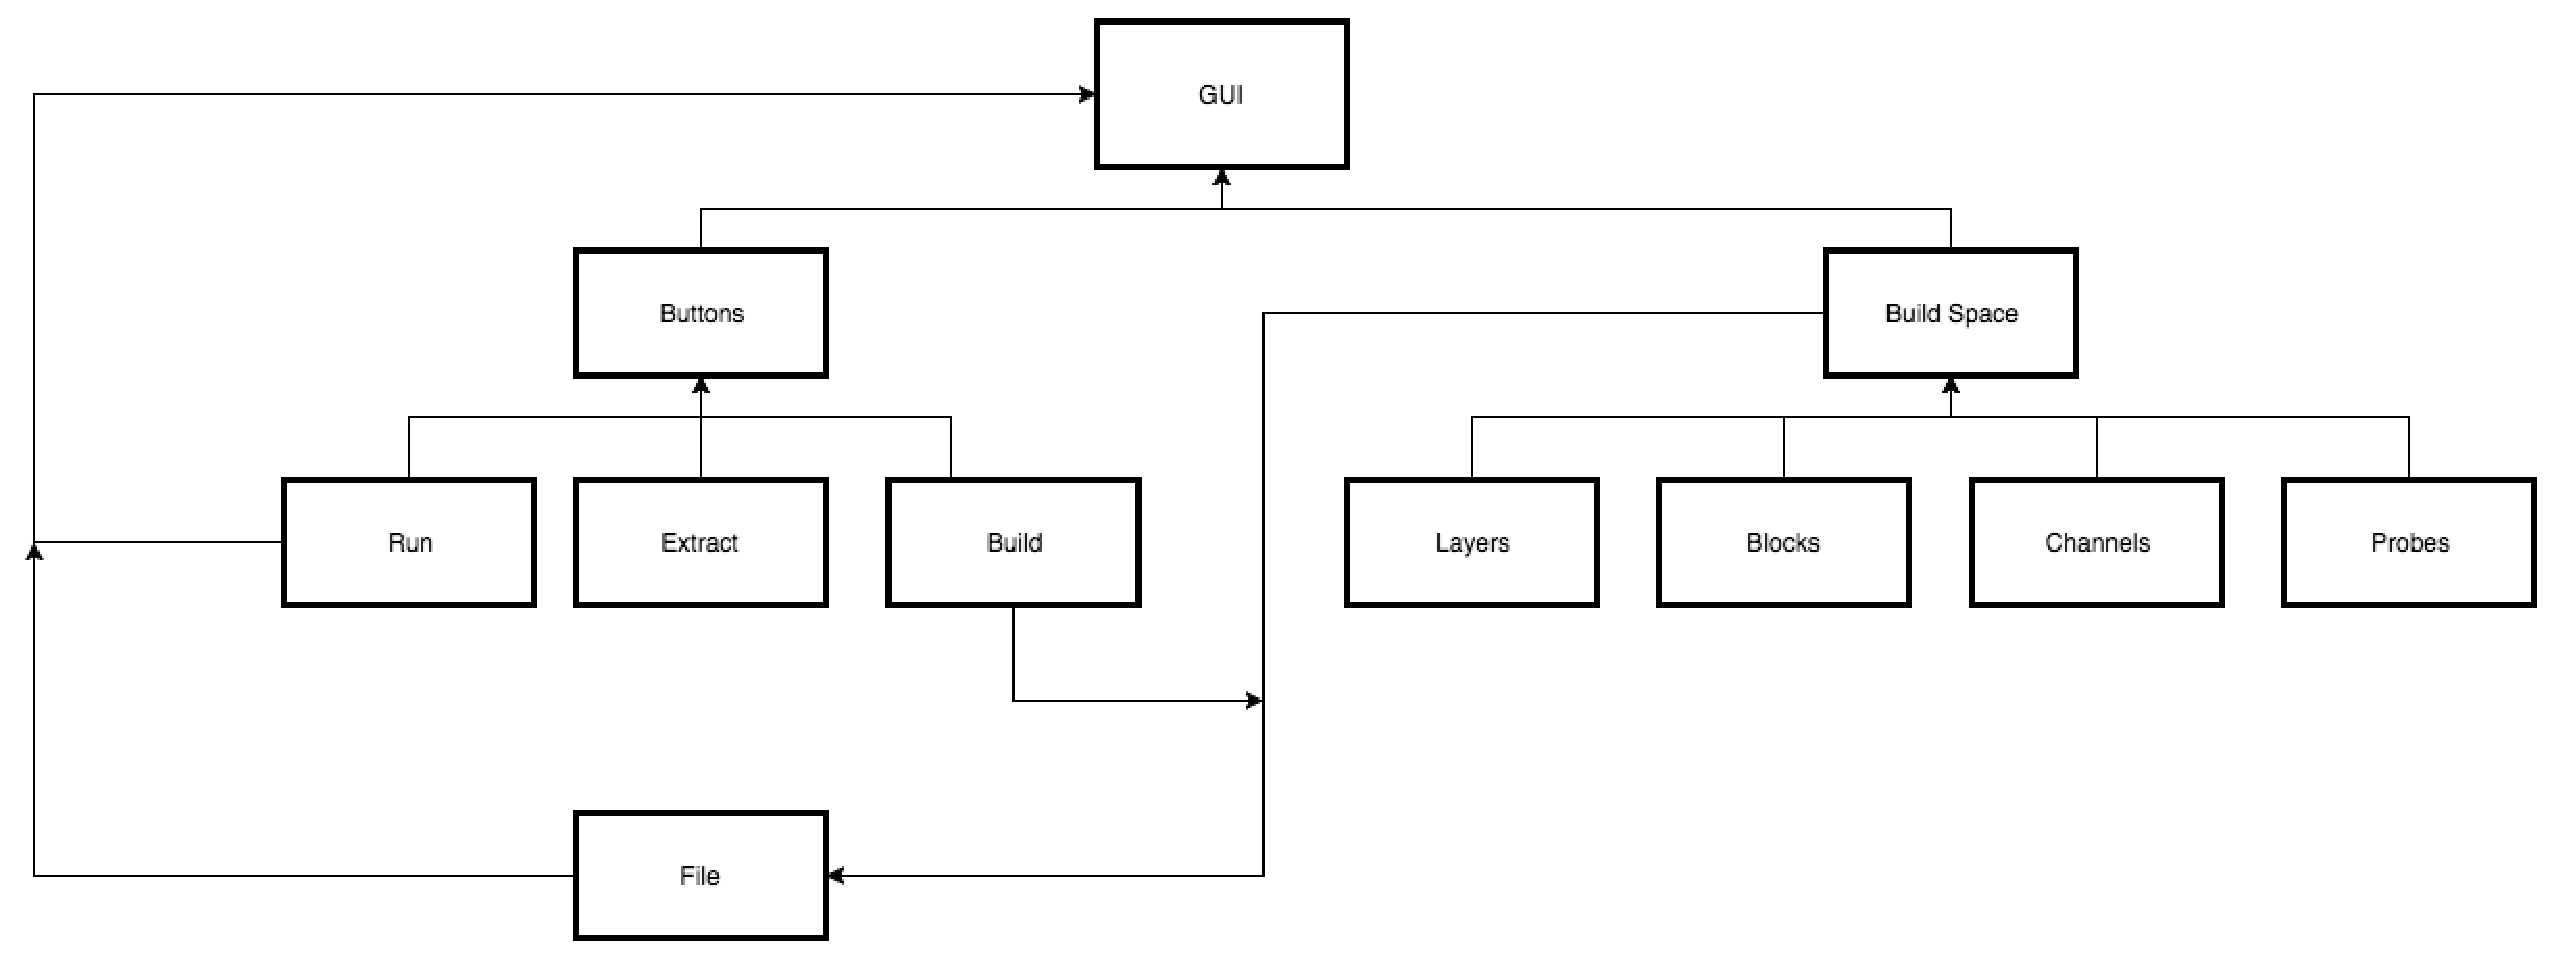
\includegraphics[width=\textwidth]{graphics/visualFlow.eps}}
\caption{Basic Architecture}
\end{figure}

\noindent The application will consist of a single main page where the user can build their program. 
This main page will feature a building area that contains the visual representation of the user's program in a flowchart-style design. 
Blocks will be located in a sidebar that lists all available features the user can utilize. 
Users can drag and drop various Blocks from the sidebar into the building area to construct their program. 
Finally, a toolbar will allow the user to create a new program, save their current program, run/stop their program, extract their program, and edit settings. 

\noindent Once the user has constructed their program in the building area and have selected the run option from the toolbar, the application will utilize TensorFlow\texttrademark API to produce a result following the user's program. During this time, the user has the ability to monitor various parameters and variables as they pass through the program.

\subsection{Decomposition Description}
\begin{figure}[H]
\fbox{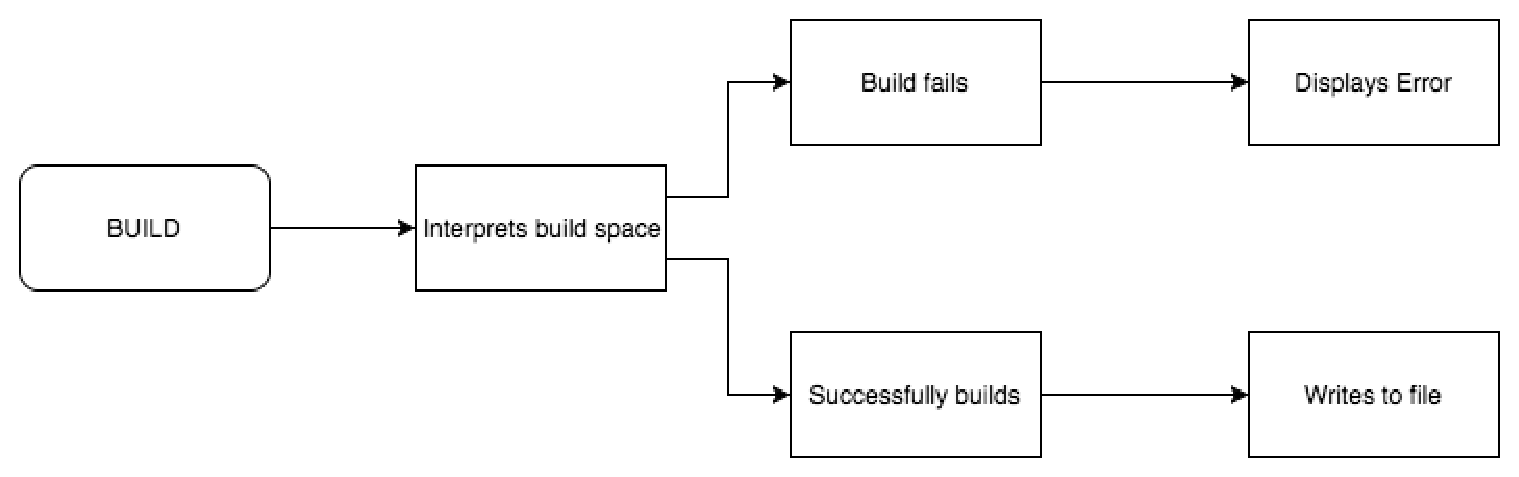
\includegraphics[width=\textwidth]{graphics/Build.eps}}
\caption{Build function}
\end{figure}

In order for users to have executable and exportable files they must have their designs turned into files by some interpreter.
The Build function is responsible for interpreting the design of the user's software.

\begin{figure}[H]
\centering
\fbox{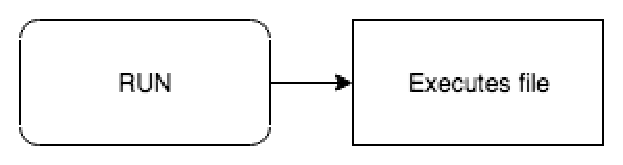
\includegraphics{graphics/Run.eps}}
\caption{Run function}
\end{figure}

\noindent To test the design of a user's software, the system must be able to put it through testing.
By using the Run feature, users are able to execute their program and check that it is working appropriately.

\begin{figure}[H]
\centering
\fbox{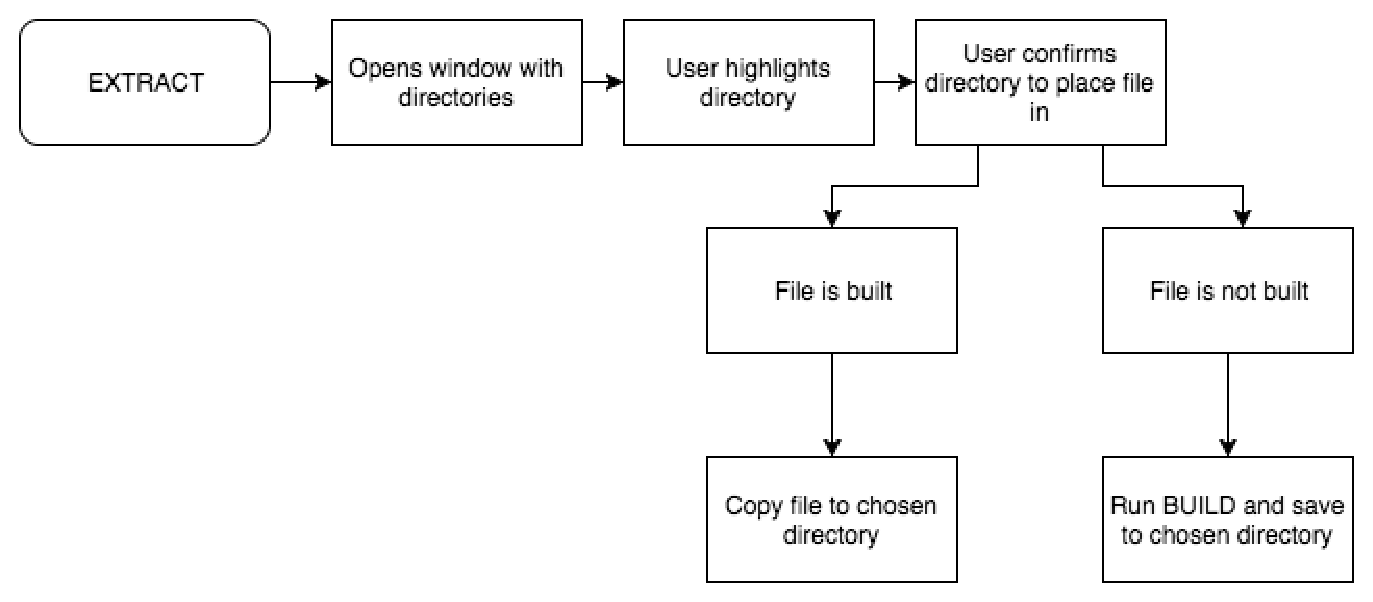
\includegraphics[width=\textwidth]{graphics/Extract.eps}}
\caption{Extract function}
\end{figure}

\noindent The functionality of the Extract feature is to create a copy of the interpreted design created by the user. 
The user is given the ability to choose where they wish to save the copy.

\begin{figure}[H]
\centering
\fbox{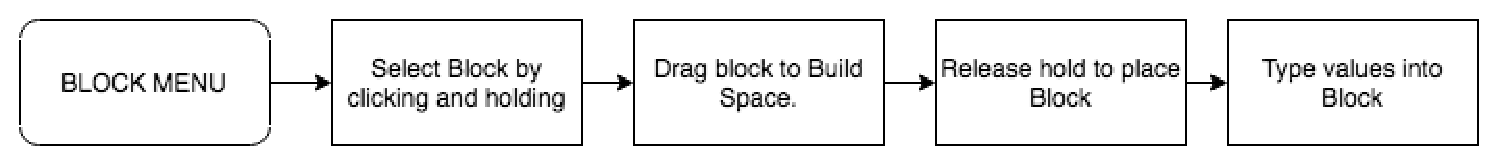
\includegraphics[width=\textwidth]{graphics/BlockMenu.eps}}
\caption{Blocks function}
\end{figure}

\noindent The function of the Blocks within the Block menu is to represent code syntax such as functions and variables.
Blocks are placed in the build space and are interpreted or translated by the build function to create files.

\begin{figure}[H]
\centering
\fbox{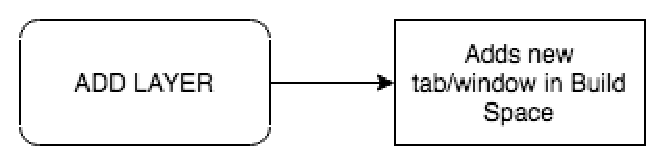
\includegraphics{graphics/Layerdiag.eps}}
\caption{Layer function}
\end{figure}

\noindent Layers sit in the build space and represent chunks of code.
Their functionality is to assist in design organization.

\begin{figure}[H]
\centering
\fbox{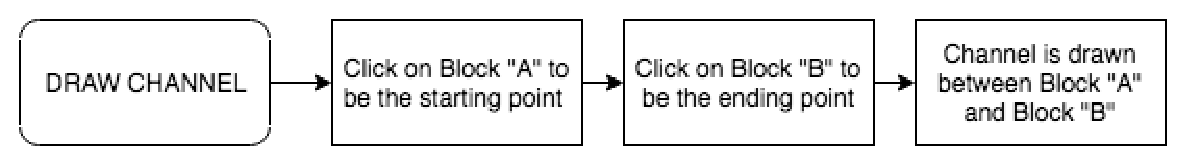
\includegraphics[width=\textwidth]{graphics/Channel.eps}}
\caption{Channel function}
\end{figure}

\noindent Channels display dependencies. 
For example, a function Block relies on a variable Block as input, as such a Channel is drawn from the variable Block to the function Block to symbolize this relationship. 

\begin{figure}[H]
\centering
\fbox{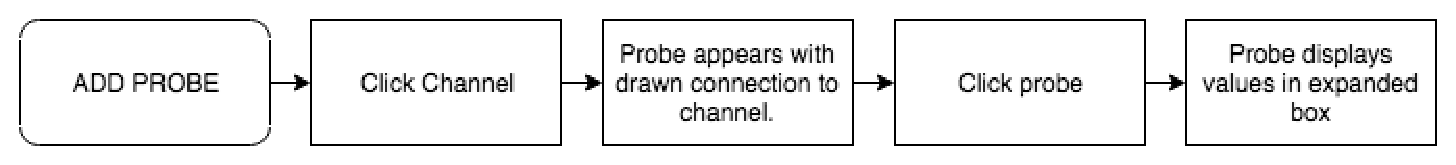
\includegraphics[width=\textwidth]{graphics/Probe.eps}}
\caption{Probe function}
\end{figure}

\noindent Probes sit on Channels. 
The function of Probes is to display the values being passed through Channels.
The purpose of this feature is to aid in debugging and variable tracking.
%---------------------------------------------
\subsection{Design Rationale}
\noindent The goal of the application is to keep user interaction as straightforward as possible so that the user can build their own program with ease. 
We hope to create this simple WYSIWYG environment by keeping all application features and operations on a single page. 
Additionally, this particular approach gives us some room for more development later on as needed. 
For example, if we want to create more Blocks for the application, we can simply add them to the sidebar and handle the implementation on the back-end. 
This same idea can also be applied to the toolbar, should more options be necessary.

\noindent Finally, the build area will utilize a flowchart-style design, allowing the user to easily recognize parameters and Blocks of their program. 
This particular design will also allow the user to quickly debug their program should any error occur, as most parameters and Blocks are quite distinct from each other.
\newpage
%---------------------------------------------
\section{TensorFlow\texttrademark WYSIWYG GUI in Perspective}\label{TWYSIWYGGUI}
%---------------------------------------------
\subsection{Design Stakeholders and their Concerns}
%\subsection{Design Views} Not sure the difference between this and viewpoints
\noindent Pertaining to the concerns of the development team, the software should be modular and easy to maintain for developer purposes. 
The reason being that the development team may wish to add features to later versions of the product.
The software should be developed in a programming language that is supported on multiple software environments.
The software should support the TensorFlow\texttrademark API.
\\ \\
\noindent Pertaining to the concerns of the user, the software should remain easy and simple to use. This is so the user can effectivly produce a program without needing to worry about the complex features of TensorFlow\texttrademark API. 
%---------------------------------------------
\subsection{Design Viewpoints}
This section describes some of the viewpoints that were applicable to the TensorFlow\texttrademark WYSIWYG graphical user interface solution. 
These viewpoints are context, interface, structure and interaction view points.
%---------------------------------------------

\subsubsection{Context Viewpoint}
\noindent When developing the TensorFlow\texttrademark WYSIWYG GUI components it is important to consider that they satisfy the stakeholder's requirements on an abstract level. 
Individuals using this software vary greatly with experience around computers. 
As such, ensuring that the interface caters to individuals with limited programming experience allows for greater marketability as a teaching tool as well as an easy-to-use developer tool.

%------------------------------------------------
%\subsubsection{Design Concerns}
%\noindent
%\subsubsection{Design elements}
%\noindent
%------------------------------------------------
%\subsubsection{Dependencies viewpoint}
%\noindent This section describes the relationship of smaller components of TensorFlow\texttrademark WYSIWYG GUI and how they are interconnected. This section dictates the implementation of most of elements in this project. This is due to the inter-connectivity of this components.

%\subsubsection{Design Concerns}
%\noindent
%\subsubsection{Design elements}
%\noindent
%------------------------------------------------
\subsubsection{Interface viewpoint}
\noindent Users will require an interface that effectively translates their software design into syntax which is readable and executable by their computer's operating system. 
Users should not have to worry about correct syntax when piecing together their programs. 
This will allow users to focus more on the relationships between Blocks and the flow of their program rather than the language behind it.

%\subsubsection{Design Concerns}
%\noindent
%\subsubsection{Design elements}
%\noindent
%------------------------------------------------
\subsubsection{Structure viewpoint}
\noindent From a viewpoint as a developer creating this software, it makes sense to develop parts in a modular format. 
This can be done by making components independent objects. 
This means granting each component its own organization and inner working elements.
This makes the structure of the software easy to manipulate during development.

%\subsubsection{Design Concerns}
%\noindent
%\subsubsection{Design elements}
%\noindent
%------------------------------------------------
\subsubsection{Interaction viewpoint}
\noindent The solution was designed to minimize each components interaction with others and maximize the independence of each component.
However, each element in this solution is still designed to interact with other components in a specific way. 
The channels in this solution make interaction of each part possible.

%\subsubsection{Design Concerns}
%\noindent
%\subsubsection{Design elements}
%\noindent
%-------------------------------------------------

\newpage

%\section{Design Viewpoints}
%------------------------------------------------
\section{Component Design}
\noindent This section will explain the details of each component used in the TensorFlow\texttrademark WYSIWYG graphical user interface. This part explains each part in three levels. These levels are the graphical user interface perspective, structural element and the design rationale.

\subsection{Scene}
\subsubsection{GUI element}
\noindent Scene is a work space that all the other features will show up on. 
This section is colored gray and its purpose is to show a significant border on where user can drag Blocks.
\begin{figure}[H]
\fbox{\includegraphics[width=\textwidth]{graphics/Capstone.eps}}
\caption{Build Space with development}
\label{fig:Capstone}
\end{figure}
\subsubsection{Structural element}
\noindent This portion is completely visual and does not have much code implementation. 
This section does not modify or affect any of the variables, classes or functions.
This section in structure will only be a square with a distinct color that separates the drag-able area from the rest of the graphical user interface.
This part needs to be extremely simple and easy to understand to prevent any confusion. 
Items which need to be considered in this design is:
\begin{itemize}
	\item \textbf{Color}: The color needs to be distinct from the rest of the elements and not too bright. 
    \item \textbf{Borders}: The borders need to be distinct and easy to spot.
    \item \textbf{Size}: The size needs to be large enough for the user to feel comfortable using it. It needs to have enough space for the user to put down ad many blocks as he needs.
\end{itemize}
\subsubsection{Design rationale}
\noindent Even though this portion is a very small in implementation, it is actually a very important part of the entire graphical user interface. 
From a user's viewpoint, this offers an abstracted view of the file that they are writing their program on.
%-------------------------------------------------
\subsection{Block}
\subsubsection{GUI element}
\noindent The Block is represented as a shape that is movable by the user within the Scene. This block makes methods, variables and classes possible in our implementation.

\subsubsection{Structural element}
\noindent Blocks are abstracted objects representing Python code syntax.
These blocks could be classified as:
\begin{itemize}
	\item \textbf{Data}: This portion is responsible for data handling in the document. (please refer to section \ref{Data})
    \item \textbf{Methods}:
    \item \textbf{Probes}:
    \item \textbf{Class}:
\end{itemize}
Blocks interact with the Scene by representing the raw code whereas the Scene represents the file that contains the code.
\subsubsection{Design rationale}
\noindent The rationale behind this design choice is that the stakeholder wants projects to be represented in a flowchart diagram format.
Flowcharts consist of Blocks or nodes which represent either actions, inputs, or outputs.
From a user viewpoint, by representing functions, variables, and classes in this manner the user is able to better visualize the architecture of their program.
From a developer viewpoint, by making each Block a modular abstraction of Python code it allows for better maintainability.

%-------------------------------------------------
\subsection{Build}
\subsubsection{GUI element}
\noindent The Build feature is a button placed in the top-left menu of the graphical user interface.This  button will build the underlying Python source.
\subsubsection{Structural element}
\noindent When clicked, the Build button will communicate to a suite of functions called getBlockType(), translateBlock(), addArguments() to interpret the Block objects in the Scene object and translate their contents into function calls and variable initialization calls.\cite{pythonvar}\cite{pythonfunction}
\subsubsection{Design rationale}
\noindent From a developer viewpoint, making this into a suite of independent functions allows this feature to be more easily maintained.

\noindent As a user, instead of worrying about syntax, they need only trust the system to do the work for them to create their file.
%-------------------------------------------------
\subsection{Block Menu}
\subsubsection{GUI element}
\noindent The Block Menu sits on the left side of the  containing instances of variable, class, and function Blocks. It is originally empty on its lower half and only contains the block types available.Every time an a type button is clicked on, it loads and shows all the available individual blocks from that type in the empty half for user to select.
Last but not least, the blocks are represented in an alphabetical order.
\subsubsection{Structural element}
\noindent This section is where other elements are dragged from.
This portion essentially spawns the blocks into the scene. 
However, this functionality does not modify the content of the block itself.
\subsubsection{Design rationale}
\noindent From a usability perspective, there was a need for an elegant way to display the blocks for selection and use in the project. This flexible solution provides an organized way of displaying all of the blocks elegantly while keeping it easy to find and navigate.
%-------------------------------------------------
\subsection{Run}
\subsubsection{GUI element}
\noindent The Run feature is a button placed in the top-left menu of the graphical user interface. This button runs the program from the underlying Python source.
\subsubsection{Structural element}
\noindent The Run feature should communicate the command "python $\langle$filename.py$\rangle$ $\langle$appropriate flags$\rangle$" to the user's system and execute the user's file.
This is done with help of the Kivy framework API to communicate commands to the system from onclick ques.\cite{Kivy}
\subsubsection{Design rationale}
\noindent From a user's viewpoint, having the execution of a file simplified to the click of a button saves time. 
This feature also makes work easier for individuals with limited technical knowledge.
%-------------------------------------------------
\subsection{Stop}
\subsubsection{GUI element}
\noindent The Stop feature is a button placed in the top-left menu of the graphical user interface. This feature brings the execution of underlying Python source to a halt.
\subsubsection{Structural element}
\noindent The Stop feature should communicate the command "ctrl C" to the user's system and end execution of a user's program.
This is done with help of the Kivy framework API to communicate commands to the system from onclick ques. \cite{Kivy}
\subsubsection{Design rationale}
\noindent From a user's viewpoint, the Stop feature makes it easy for them to end execution of their program.

\noindent From a developer viewpoint, this makes it simple to implement a feature that stops execution of a file.
%-------------------------------------------------
\subsection{Extract}
\subsubsection{GUI element}
\noindent The Extract feature is a button placed in the top-left menu of the graphical user interface.
\subsubsection{Structural element}
\noindent The Extract feature allows the user to save a copy of their program onto their personal computer or device.  
This is done with help of the Kivy framework API to communicate commands to the system from onclick ques.\cite{Kivy}
\subsubsection{Design rationale}
\noindent Allowing the user to extract their current project gives them the ability to use a stand-alone version of the program.
%-------------------------------------------------
\subsection{Variable/Constant Blocks}
\subsubsection{GUI element}
\noindent The Variable and Constant Blocks are represented as rhombuses. 
They can be dragged and dropped onto the Scene.
\subsubsection{Structural element}
\noindent Variable/Constant Blocks are Python objects with attributes.\cite{pythonvar}\cite{pythonclass}
These attributes are "Block\_type", "value", and "name."
\subsubsection{Design rationale}
\noindent From a developer viewpoint, this method makes it easier to model Blocks as lines of code to be interpreted by the Build functions.
%-------------------------------------------------
\subsection{Method Blocks}
\subsubsection{GUI element}
\noindent Method Blocks are represented as rectangles.
They can be dragged and dropped onto the Scene.
\subsubsection{Structural element}
\noindent Variable/Constant Blocks are Python objects with attributes.\cite{pythonfunction}\cite{pythonclass}
These attributes are "Block\_type", "Arguments[]", and "Name."
\subsubsection{Design rationale}
\noindent From a developer viewpoint, this method makes it easier to model Blocks as lines of code to be interpreted by the Build functions.
%-------------------------------------------------
\subsection{Class Blocks} 
\subsubsection{GUI element}
\noindent Class Blocks are represented as squares.
They can be dragged and dropped onto the Scene.
\subsubsection{Structural element}
\noindent Class Blocks are Python objects with attributes.\cite{pythonclass}
These attributes are "Block\_type", "Attributes[]", and "Name."
\subsubsection{Design rationale}
\noindent From a developer viewpoint, this method makes it easier to model Blocks as lines of code to be interpreted by the Build functions.
%-------------------------------------------------
\subsection{Abstract}
\subsubsection{GUI element}
\noindent The Abstract feature is a feature that allows the user to draw a box over their Blocks to mask their contents. 
Using this feature also nullifies any Probes within the drawn area.
\subsubsection{Structural element}
\noindent The Abstraction feature does not affect the underlying interpretation of the code Blocks by the Build feature and its underlying functions.
\subsubsection{Design rationale}
\noindent From a user's viewpoint, the Abstraction feature can assist the user in covering up or labeling certain chunks of their code to assist them in making their software design more modular, easier to read, and organized.
%-------------------------------------------------
\subsection{Layer}
\subsubsection{GUI element}
\noindent The Layer component puts all the Layer elements in a visual queue for user to be able to see them. Furthermore, it allows users to interact with their "layer" level inputs and outputs.\\
\begin{figure}[H]
\fbox{\includegraphics[width=\textwidth]{graphics/Layer.eps}}
\caption{Layering system}
\label{fig:inLayer}
\end{figure}
\noindent This component provides drag-able elements to identify inputs and outputs to each Layer. 
Furthermore, it allows for addition and deletion of Layers.
\subsubsection{Structural element}
\noindent The concept behind Layers is to separate certain conceptual levels in a machine learning application architecture. 
Each layer may contains many other GUI elements. 
Furthermore, Layers could be named and identified with tags for better representation, organization and ease of navigation.
\subsubsection{Design rationale}
\noindent Our client requires this feature to aid in organizing the build space.
This approach is present in many machine learning and computer vision software designs and separates core stages of the software.
\subsubsection{Abstraction}
\noindent For having a better view over this element, please refer to Abstraction subsection. 
This functionality is also available to Layers with small difference. 
The abstraction option of a Layer is only for cleanliness and does not have any affect on the implementation of the actual Layer components. 
All it does is mask the content of the Layer for visibility and navigation purposes.
%-------------------------------------------------
\subsection{Channel}
\subsubsection{GUI element}
\noindent The Channel is a feature connecting vital Blocks components. The channels are where the data flows and they indicate the data flow with arrows.
\subsubsection{Structural element}
\noindent They connect outputs of blocks to inputs of others. The channels are one directional and data only flows in one way within the channels. in code level the channels are just place holders indicating which variable needs to be filled in for other method arguments.
\subsubsection{Design rationale}
\noindent This WYSIWYG solution needs a mean of connecting all the blocks to one another. Visually displaying the route that inputs and outputs take will give the user an easier understanding of the data flow in their program. This means that user can quickly identify any issues/problems and apply fixes as needed. This concept is represented with lines in figure \ref{fig:Capstone}
%-------------------------------------------------
\subsection{Probe}
\subsubsection{GUI element}
\noindent The Probe is a feature placed on Channels between different Block elements. The Probe feature is a Block type that displays the current input and output content of a Channel. Users can modify the value being transmitted through the Channel. If the value of a Probe is modified, the modification will happen after the point which the probe is inserted into the Channel.
\subsubsection{Structural element}
\noindent This portion interacts with channels specifically. In implementation level it just displays the data and it is also capable of modifying the data in the channel. Furthermore, from a GUI perspective, it only modifies the data after the connection point to the channel (represented by blue transparent circle in figure \ref{fig:Capstone}).
\subsubsection{Design rationale}
\noindent The idea of the Probe is to give the user additional debugging techniques as well as the ability to visually see where individual inputs and  outputs occur in the program.
%-------------------------------------------------
\subsection{Data}\label{Data}
\subsubsection{GUI element}
\noindent The data button is designed to represent all the input types that our solution supports. The data elements have 1 input and 1 output with the exception of pointer element which has 2 inputs and 2 outputs. The inputs modify and the outputs connect to channels to return their value.
Lastly, these blocks represent the values stored in the variable at run-time.
\subsubsection{Structural element}
\begin{itemize}
	\item \textbf{Input}: This requires a type of input. That type could be keyboard stroke or files.
	\item \textbf{Variables}: This type  of data is modifiable during run-time.
    \item \textbf{Constants}: This data type is not modifiable and user cannot change the content of it in run-time. Once the code starts executing, their content stays constant.
    \item \textbf{Pointer}: This data type will not allocate any memory but rather is assigned an address. 
    Once the address is set the variable becomes modifiable.
    In this setup the address stays modifiable during run-time. As mentioned earlier, the pointer element has 2 inputs and 2 outputs. One of the inputs and outputs modify and return the value of the pointer and the other input and output modify and return the address.
    \item \textbf{Output}: Output is the end of each pipeline.
    after placement of output it does not allow for further progression of the code. The output could be in for of a value or a file.
\end{itemize}
\subsubsection{Design rationale}
\noindent The WYSIWYG solution needs a mean of representing the data itself. This could be in form of blocks that display that value and allow the modification of those values (please see figure \ref{fig:Data}). 
%-------------------------------------------------
\newpage
\section{User Interface Design}
\subsection{Overview of User Interface}
\noindent The user interface of TensorFlow\texttrademark WYSIWYG Graphical User Interface is designed to remain as simple as possible for the user. 
This is to ensure that they can effectively create, organize, and debug their program. 
To start, the user will be presented with a building area where they can place different Block elements and features. 
A sidebar featuring a list of the various Blocks available will allow the user to easily drag and drop these Blocks into the building area. 
Each individual Block is unique in that they give the user a visual representation of a particular aspect of the TensorFlow\texttrademark API. 
The building area can be broken down into separate Layers, which represent different aspects of the user's program. 
This gives the user additional control over the flow of their program. 
Finally, a toolbar at the top of the application will give the user various options. 
Such options include the ability to run the program, save progress on the current program, or extract the program for stand-alone use.
\subsection{Screen Images}
\begin{figure}[H]
\fbox{\includegraphics[width=\textwidth]{graphics/Basic-1.eps}}
\caption{Basic interface scheme}
\label{fig:Basic}
\end{figure}

\begin{figure}[H]
\fbox{\includegraphics[width=\textwidth]{graphics/Data.eps}}
\caption{Block Menu visible}
\label{fig:Data}
\end{figure}

\begin{figure}[H]
\fbox{\includegraphics[width=\textwidth]{graphics/Capstone.eps}}
\caption{Build Space with development}
\end{figure}

\begin{figure}[H]
\fbox{\includegraphics[width=\textwidth]{graphics/Abstract.eps}}
\caption{Data structure abstraction}
\label{fig:Abstract}
\end{figure}

\begin{figure}[H]
\fbox{\includegraphics[width=\textwidth]{graphics/Layer.eps}}
\caption{Layering system}
\label{fig:outLayer}
\end{figure}

\subsection{Screen Objects and Actions}
\begin{itemize}
	\item \textbf{Scene}: On its own, the scene does not offer the user any sort of action or functionality.
    The scene simply acts as a container which holds all of the elements and features of the user's program.
    Once Blocks are placed in the scene, the user can interact with and move these Blocks in order to structure their program as they see fit.
    \item \textbf{Block Menu}: The Block Menu acts as a list containing all of the various Block types the user can utilize for their program.
    Located on the left side of the application, users can easily drag and drop the desired Blocks into the scene. 
    \item \textbf{Toolbar}: Like the Block Menu, the Toolbar contains a list of various functions the user can utilize.
    These functions include actions such as saving the user's program, loading a new program, or starting and stopping the current program.
    Located at the top of the application, the user simply needs to select and click on one of these options for the function to take effect. 
\end{itemize}

\newpage
\bibliographystyle{IEEEtran}
\bibliography{sources}
\end{document}
